\documentclass{article}
\usepackage[utf8]{inputenc}
\usepackage{tikz}

\title{Module System}
\author{Fin}
\date{September 2021}

\begin{document}

\maketitle

\section{Introduction}
The module system I'll describe here has only one goal: Scalability.
I'll say scalability is achieved when the amount of context that a programmer needs to be aware of when working on a module is independent of the scale of the codebase.

The terminology I'll use here is a mix of computer science jargon and graph theory jargon. There is a name collision for "Module". In this article a Module means a file. When represented in the graphs the module is a single node.

To get a clear view of the options for which modules import which, all programs will be visualized as directed graphs. 
The vertices are modules.
The edges represent one module importing another 
The module at the end of the arrow is the importing module. 
The module at the start of the arrow is the module being imported. 
The reason why the module system will be explained using graph theory is because graph theory is a good model to describe and visualize this particular kind of module system. Another reason is that we can also abstract away from the actual module system and just think about graphs when this is necessary. It comes in handy when you want to be sure every form of module system (under graph theory constraints) has been considered.


The method to get to the resulting module system is as follows:

\begin{enumerate}
    \item Take the graph for a module system where different nodes
(representing modules) have a rough constant amount of context unrelatable to the size of the graph. The amount of \emph{possible} edges to be drawn should be as small as possible.

    \item Look at the problems this poses in terms of actually constructing programs under those constraints. Then see how these problems can be solved while still keeping as many constraints on the edges as possible.
    
    \item Iterate on step 2, if no problem was found then we’ll stop iterating and take the module system as done.
\end{enumerate}

%---------------------------------------------------------------------------%
%---------------------------------------------------------------------------%
%---------------------------------------------------------------------------%
%---------------------------------------------------------------------------%
%---------------------------------------------------------------------------%
%---------------------------------------------------------------------------%
%---------------------------------------------------------------------------%
%---------------------------------------------------------------------------%
%---------------------------------------------------------------------------%
%---------------------------------------------------------------------------%

\section{Building Programs With Trees}

The most restrictive model which is scalable, is a tree. 
In a tree, each node only has to worry about the effect on its parent, and the only “tools” a node needs to know about are its children and the core programming language itself.

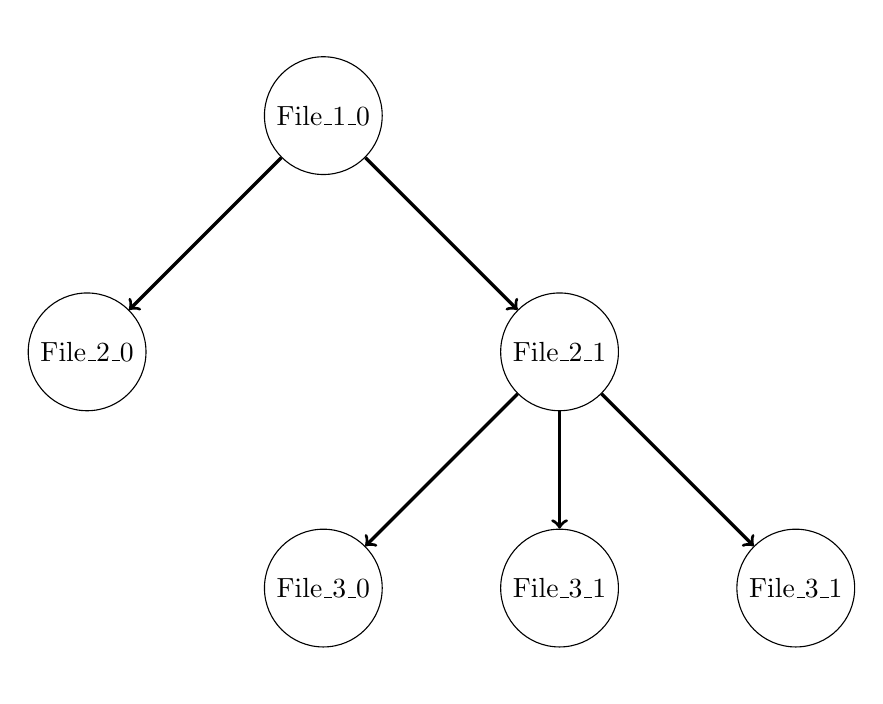
\begin{tikzpicture}

%SPACING
\node[](v0) at (0,8) {};
%SPACING

\node[circle,draw=black](v1) at (3,7) {File\_1\_0};
\node[circle,draw=black](v2) at (0,4) {File\_2\_0};
\node[circle,draw=black](v3) at (6,4) {File\_2\_1};
\node[circle,draw=black](v4) at (3,1) {File\_3\_0};
\node[circle,draw=black](v5) at (6,1) {File\_3\_1};
\node[circle,draw=black](v6) at (9,1) {File\_3\_1};

%SPACING
\node[](v7) at (0,0) {};
%SPACING

\draw[->,very thick] (v1) -- (v2);
\draw[->,very thick] (v1) -- (v3);

\draw[->,very thick] (v3) -- (v4);
\draw[->,very thick] (v3) -- (v5);
\draw[->,very thick] (v3) -- (v6);

\end{tikzpicture}

In this example, File\_2\_1 only needs to worry about its effect on File\_1\_0. In other words: When File\_2\_1 changes the implementation of a function for instance, it only needs to make sure that File\_1\_0 (the only module that can import that function) still behaves correctly. Of course it also needs to make sure the module itself (in this case File\_2\_1) isn’t affected badly, but since that is always a factor, no matter how the module system works, I won’t talk about that, just keep it in mind.

The only tools that File\_2\_1 needs to worry about is what the children modules export (functions, types, macros, ...). And of course the language itself is also a tool available. But then again, the (core) language itself will always be a tool, no matter what the module system looks like. So again I also won’t mention that factor anymore, just keep it in mind.

In theory this module system works great! No matter how large the program already is, the programmer will only need to keep in mind a certain amount of context which is independent of the size of the program. That context is:

\begin{enumerate}
    \item The influence of the developed module on the parent.
    \item The tools provided by the children of the developed module.
\end{enumerate}

%---------------------------------------------------------------------------%
%---------------------------------------------------------------------------%
%---------------------------------------------------------------------------%
%---------------------------------------------------------------------------%
%---------------------------------------------------------------------------%
%---------------------------------------------------------------------------%
%---------------------------------------------------------------------------%
%---------------------------------------------------------------------------%
%---------------------------------------------------------------------------%
%---------------------------------------------------------------------------%

\section{Adding Libraries}

There is something that bugs me about this way of structuring programs though. That is that there is no way of reusing code! In theory the programmer will always only have to worry about the context specified in Section 1, in reality that’s hard to achieve and wrong assumptions will be made. Let me illustrate this with an example:

"\emph{Say a programmer has a strcmp() function. This function takes two strings, and returns 1 if the former is bigger, 0 if they are both equal, and -1 if the former is smaller. Since there is no way to reuse code, the programmer will copy paste this function quite a lot. One day another programmer joins the team, and he too needs to compare two strings. He’s not aware of the already existing code for strcmp() in the codebase, nor should he! Anyways, the programmer wants to know if two strings are equal. If they are equal, he makes his strcmp() return 1, else it returns 0. Now a third programmer joins the team and scrolls through the codebase. He’ll find inexplicable behaviour because when he sees a strcmp in the code, it’ll sometimes mean one thing, and other times it’ll mean another thing. He can’t really see the “correct” implementation of strcmp(), because there isn’t one “correct” implementation, there are multiple!}"


Yes, in theory every programmer should get familiar with the correct context and only that context first before reading code in a module, but in reality assumptions will be made, and it will be a human source of error that could be avoided if there was some way of reusing code. Besides, even though it would theoretically be a “scalable” approach to software construction, it’s unnecessarily tedious and the lack of code reuse makes for incredibly slow progress.


That is why a separate folder, independent from the project structure, should be made. In that folder go all the libraries, and a library can be imported from any module. This way a programmer has two options:

\begin{enumerate}
    \item Add a module to the project. When writing/changing code in this module, the programmer knows what influence it has, namely the parent.
    \item Add a library to the Libraries folder. When writing/changing code in this library, all bets are off regarding the influence of it. Not only is it unknown how many modules are affected in the project, in the future new modules might also be needing those libraries.

\end{enumerate}


This separation makes programmers know what they’re getting into. Are they changing a module? Then the scope of the effect is known and limited, and can be checked for errors. Are they changing a library? Then they are aware that it can affect the entire program.


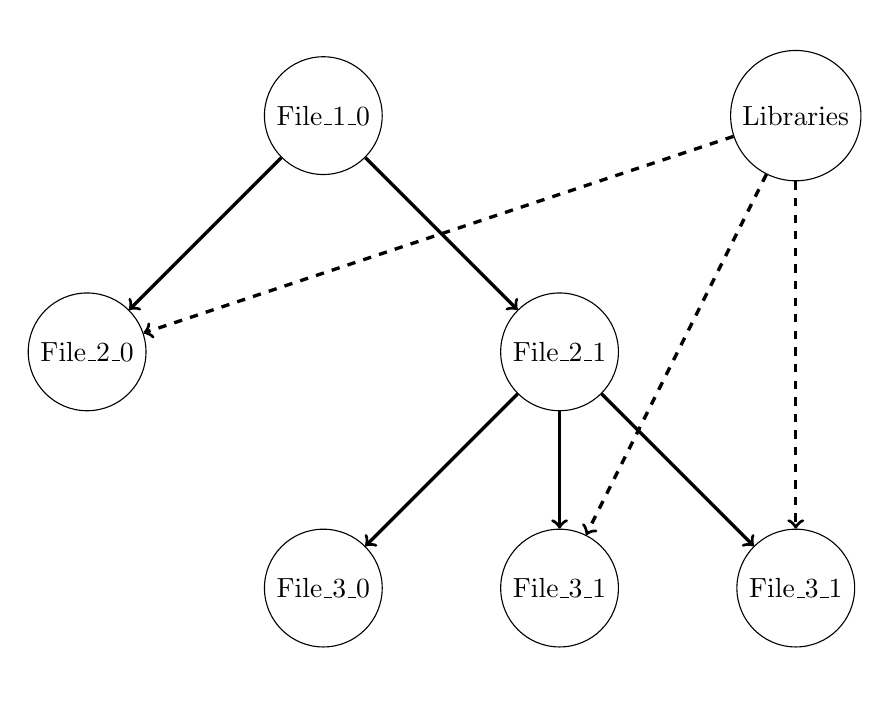
\begin{tikzpicture}

%SPACING
\node[](v0) at (0,8) {};
%SPACING

\node[circle,draw=black](lib) at (9,7) {Libraries};

\node[circle,draw=black](v1) at (3,7) {File\_1\_0};
\node[circle,draw=black](v2) at (0,4) {File\_2\_0};
\node[circle,draw=black](v3) at (6,4) {File\_2\_1};
\node[circle,draw=black](v4) at (3,1) {File\_3\_0};
\node[circle,draw=black](v5) at (6,1) {File\_3\_1};
\node[circle,draw=black](v6) at (9,1) {File\_3\_1};

%SPACING
\node[](v7) at (0,0) {};
%SPACING

\draw[->,very thick] (v1) -- (v2);
\draw[->,very thick] (v1) -- (v3);

\draw[->,very thick] (v3) -- (v4);
\draw[->,very thick] (v3) -- (v5);
\draw[->,very thick] (v3) -- (v6);

\draw[->,dashed,very thick] (lib) -- (v2);
\draw[->,dashed,very thick] (lib) -- (v5);
\draw[->,dashed,very thick] (lib) -- (v6);

\end{tikzpicture}


%---------------------------------------------------------------------------%
%---------------------------------------------------------------------------%
%---------------------------------------------------------------------------%
%---------------------------------------------------------------------------%
%---------------------------------------------------------------------------%
%---------------------------------------------------------------------------%
%---------------------------------------------------------------------------%
%---------------------------------------------------------------------------%
%---------------------------------------------------------------------------%
%---------------------------------------------------------------------------%

\section{Adding Clusters}

Yet sometimes you know that you would like a module to be included in only a finite (let’s say n) amount of other modules. In that case you’re in a pickle. You now have two options really:

\begin{enumerate}
    \item Rewrite the module n times and make it a child of those n other modules.
    \item Write the code once and put it in the Library folder.
\end{enumerate}

In the first case, you’re back to that same old problem of not reusing code where you really could and should. In the second case, you’ve made a module accessible to all modules, even those who don’t need access. If we allow the programmer to import other modules without any restriction, then pretty much every module is global, just like libraries, and then we have defeated the point of decoupling certain parts and modules of the program from each other. So we need a way of allowing us to break the restrictions of a tree, while also not ending up with every module being accessible by every other module.


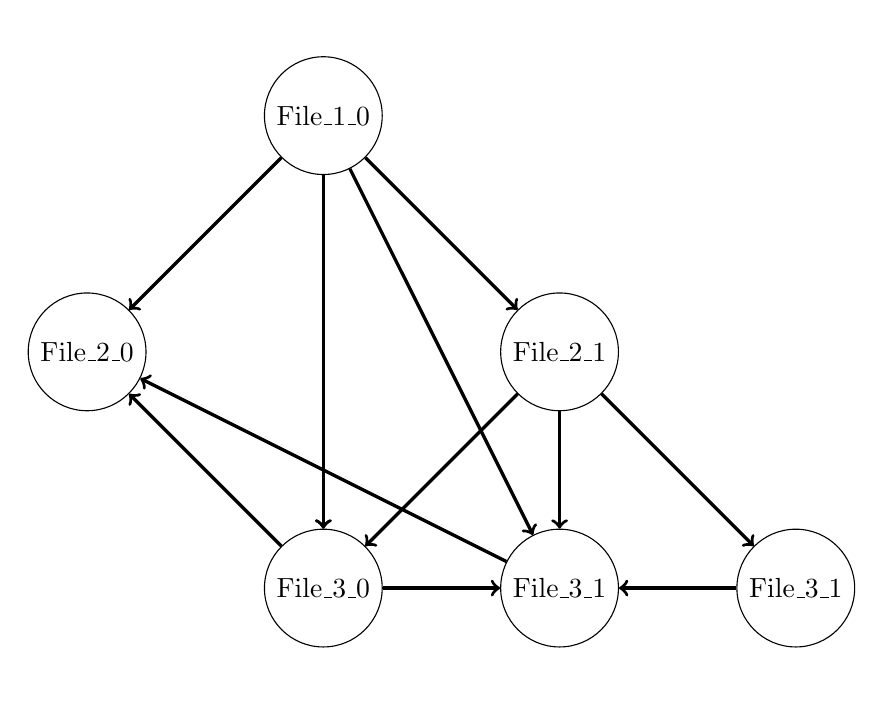
\begin{tikzpicture}

%SPACING
\node[](v0) at (0,8) {};
%SPACING

\node[circle,draw=black](v1) at (3,7) {File\_1\_0};
\node[circle,draw=black](v2) at (0,4) {File\_2\_0};
\node[circle,draw=black](v3) at (6,4) {File\_2\_1};
\node[circle,draw=black](v4) at (3,1) {File\_3\_0};
\node[circle,draw=black](v5) at (6,1) {File\_3\_1};
\node[circle,draw=black](v6) at (9,1) {File\_3\_1};

%SPACING
\node[](v7) at (0,0) {};
%SPACING

\draw[->,very thick] (v1) -- (v2);
\draw[->,very thick] (v1) -- (v3);

\draw[->,very thick] (v3) -- (v4);
\draw[->,very thick] (v3) -- (v5);
\draw[->,very thick] (v3) -- (v6);
\draw[->,very thick] (v4) -- (v5);
\draw[->,very thick] (v5) -- (v2);
\draw[->,very thick] (v6) -- (v5);
\draw[->,very thick] (v1) -- (v4);
\draw[->,very thick] (v1) -- (v4);
\draw[->,very thick] (v1) -- (v5);
\draw[->,very thick] (v4) -- (v2);

\end{tikzpicture}


The solution is clusters. Basically, they are parts of the program where modules can import each other without forming a tree hierarchy. Those parts where that breaking of the rules happens are isolated, Basically there is one parent module acting as the “interface” of the cluster, and the children modules can access each other in this cluster. Children modules normally can’t access each other in a tree, but in a cluster they can. The “interfacing” parent module is a component of another structure, either a cluster or a tree. Note that in these clusters there is still the rule that the graph must be an acyclic directed graph, in order to avoid circular dependencies.

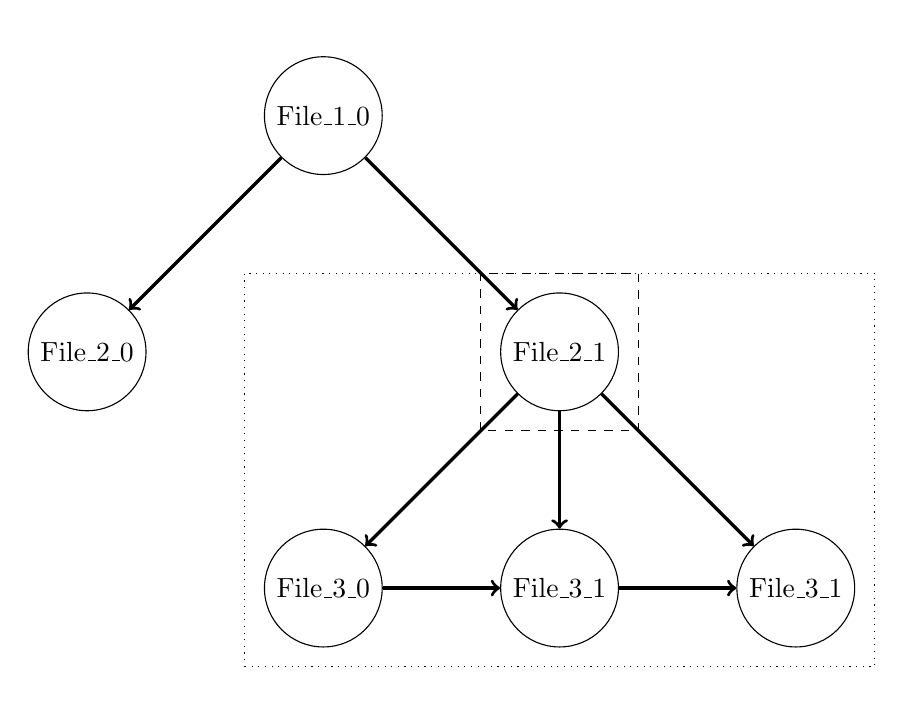
\begin{tikzpicture}

%SPACING
\node[](v0) at (0,8) {};
%SPACING

\node[circle,draw=black](v1) at (3,7) {File\_1\_0};
\node[circle,draw=black](v2) at (0,4) {File\_2\_0};
\node[circle,draw=black](v3) at (6,4) {File\_2\_1};
\node[circle,draw=black](v4) at (3,1) {File\_3\_0};
\node[circle,draw=black](v5) at (6,1) {File\_3\_1};
\node[circle,draw=black](v6) at (9,1) {File\_3\_1};

%SPACING
\node[](v7) at (0,0) {};
%SPACING

\draw[->,very thick] (v1) -- (v2);
\draw[->,very thick] (v1) -- (v3);

\draw[->,very thick] (v3) -- (v4);
\draw[->,very thick] (v3) -- (v5);
\draw[->,very thick] (v3) -- (v6);

\draw[->,very thick] (v4) -- (v5);
\draw[->,very thick] (v5) -- (v6);

\draw[dotted] (2,0) rectangle (10,5);
\draw[dashed] (5,3) rectangle (7,5);

\end{tikzpicture}


This picture shows how the “interfacing parent” is then again part of the tree structure. The cluster encapsulates modules that can use each other in random ways (as long as the result is an acyclic directed graph). The children (File4\_0, File4\_1 and File4\_2) can be an “interfacing” parent of another lower level cluster or a parent from children in another lower level tree structure.

When creating structures with clusters and subclusters there is again only a finite amount (unrelated to the size of the project) of context a programmer needs to know about when working on a module. For the interfacing parent that context is the same as for a parent in a tree. For the children of the interfacing parent that context is:

\begin{enumerate}
    \item The influence on the interfacing parent.
    \item All the other clusterchildren of the interfacing parent.
    \item Whatever subtrees/subclusters the current module is built from.
\end{enumerate}

%---------------------------------------------------------------------------%
%---------------------------------------------------------------------------%
%---------------------------------------------------------------------------%
%---------------------------------------------------------------------------%
%---------------------------------------------------------------------------%
%---------------------------------------------------------------------------%
%---------------------------------------------------------------------------%
%---------------------------------------------------------------------------%
%---------------------------------------------------------------------------%
%---------------------------------------------------------------------------%

\section{Adding Other Graph Restrictions}

So far we've looked at what kind of "subgraphs" we'd need to add. When there was a problem we faced, it became clear we needed to support less restrictive forms of graphs as well. We have covered some problems that were clear at first glance, but the question becomes: are there other problems we looked over that could benefit from another form of subgraph. We started out with trees as the "most restrictive approach for structuring projects". That was actually not the correct starting point if we really wanted to follow the process described at the start for getting to our module system. A more restrictive graph would be a list. Where each module can only import one other module, unlike a tree, where each module can import one or more modules. We've missed many graphs, and we can orient which we missed as follows:
from most to least restrictive:

... - trees - ... - acyclic graphs - ... - graphs

Before trees we could place lists, or binary trees for instance. I see no reason why those structure enforcements would benefit a project. Perhaps there are use cases, but at the same time I feel like adding them to the module system would do more harm by increasing the complexity of the module system than it would benefit by posing more constraints than a tree in a few cases.

Between trees and acyclic graphs, there could be a form of graph such as a tree with the extra possibility of parents also being able to access grandchildren. Again, This kind of enforcement seems not like it would do more good than harm when adding it to the module system.


I've covered these examples just to show that there are more graph forms than we considered. I also showed why we didn't take some other graph forms. Even though I rejected the graph forms specified above, I have admittedly not covered all possible graph forms. Who knows there might be another graph form worth adding.


%---------------------------------------------------------------------------%
%---------------------------------------------------------------------------%
%---------------------------------------------------------------------------%
%---------------------------------------------------------------------------%
%---------------------------------------------------------------------------%
%---------------------------------------------------------------------------%
%---------------------------------------------------------------------------%
%---------------------------------------------------------------------------%
%---------------------------------------------------------------------------%
%---------------------------------------------------------------------------%

\section{Trivia}

\begin{enumerate}
    \item This idea of building clusters from clusters is called “Hierarchical Modularity” in graph theory.

    \item Confusingly, modules in graph theory jargon are synonyms for clusters. Here however, the definition of a module is just a node in the graph (a file). The definition of a cluster here is a directed acyclic graph of nodes.
    
    \item It is not possible to save a project as a graph (at least as far as I know). So one might start wondering how it could be done. My solution is to have for every node a directory, containing two things:
    
    \begin{enumerate}
        \item The actual source file with the code.

        \item a directory for the children. If the children are part of the tree structure, the directory is called “TreeChildren”. If the children form a cluster, the directory is called “ClusterChildren”. Either way, that directory contains a bunch of children module nodes. Which in turn are directories containing 2 things, ... You see the recursion here that builds projects...
    
    \end{enumerate}
    
    \item The difference in use of directories here compared to how other programming languages have module systems is that the other languages just groups similar modules together, while in this language modules are grouped under restrictions and these groupings make for the structure of the program. With that being said, in the libraries folder, similar modules should be grouped together since the libraries folder doesn’t contain implementations but instead contains only “interfaces” or “declarations”. Hence the libraries folder should aid a heuristic search for the desired library module.
    
\end{enumerate}


%---------------------------------------------------------------------------%
%---------------------------------------------------------------------------%
%---------------------------------------------------------------------------%
%---------------------------------------------------------------------------%
%---------------------------------------------------------------------------%
%---------------------------------------------------------------------------%
%---------------------------------------------------------------------------%
%---------------------------------------------------------------------------%
%---------------------------------------------------------------------------%
%---------------------------------------------------------------------------%

\section{Conclusion}

This module system “works” if it is possible to keep adding code with a roughly constant amount of context to keep in mind, where the amount of context is unrelated to the scale of the program. If a module system accomplishes that, then it “works” for the purpose stated here (scalability). 


We can also say that every structure of a program can be made with the module system, since by definition the only structure that can't be made by acyclic graphs are cyclic graphs. In programming cyclic graphs introduce problems (circular dependencies), so we don't want that kind of structure for a program ever. So for all the structures a program might need, the current module system works.


Even if it works though, that doesn't mean it is perfect. For instance, if the module system hadn't trees, but only clusters built from subclusters and so on ..., then the amount of context one would need to know about would still be unrelated to the size of the program. However by adding trees we've made it so programmers need to worry about even less context in some areas of code since trees pose more constraints. So even tho a module system of only clusters "works", a module system that has also trees besides clusters is better. Following the same rationale for other graph forms it is possible that there exist better module systems that use other graph forms too. We haven't found those graph forms, but we cannot say that it is impossible that they exist.


Besides, there might be value in looking for a module system which is more user friendly in some way. Although the priority here is scalability, there might be other kinds of module systems (perhaps OOP if done correctly) which provide scalability along with other benefits.

Even though I don’t want to restrict the search for better module systems to be in the bounds of graph theory, I also believe that module systems that fit graph theory are an untapped area and so it shouldn’t be ignored.


\end{document}
